\section{Measurement and Characterization of the Reciprocal Standard}
\label{sec:ch5_reciprocal}

Unlike SOLT or TRL, the SOLR framework does not require the fourth standard to be an ideal zero-length thru or a fully characterized line. Instead, after the reflection behavior is established by the Short, Open, and Load standards, the remaining information is supplied by a two-port standard whose defining property is reciprocity. The sole reciprocity requirement is especially important in the present four-port probing geometry, since an adjacent-port connection is necessarily non-collinear and therefore cannot be treated as an ideal thru. A measured reciprocal structure with sufficiently low loss, smooth phase behavior, and close forward/reverse symmetry is therefore the physically meaningful fourth standard for the later SOLR implementation \cite{solr_patent_2010,Daniel2005USF,shakya2025_apmc}.

The fabricated die includes three through-like structures relevant to this role: a straight Thru, an arc Thru, and a diagonal Thru. The straight Thru serves as the best-controlled collinear reference and was already used in Section~\ref{sec:measured_sol_standards} to identify the common embedding from the probe-tip reference plane to the standard-definition plane.
\begin{equation}
\mathbf{A}_{\mathrm{thru,meas}}(f)=\mathbf{A}_{E}(f)\,\mathbf{A}_{L}(f)\,\mathbf{A}_{E}(f),
\label{eq:recip_thru_embed}
\end{equation}
where \(\mathbf{A}_{L}(f)\) is the explicit \(25.44~\mu\mathrm{m}\) center-line model and \(\mathbf{A}_{E}(f)\) is the common embedding extracted from the measured straight Thru. Once \(\mathbf{A}_{E}(f)\) has been identified, any reciprocal candidate can be referred to the same standard-definition plane through
\begin{equation}
\mathbf{A}_{R,\mathrm{meas}}(f)=\mathbf{A}_{E}(f)\,\mathbf{A}_{R}(f)\,\mathbf{A}_{E}(f),
\label{eq:recip_meas_embed}
\end{equation}
or equivalently,
\begin{equation}
\mathbf{A}_{R}(f)=\mathbf{A}_{E}^{-1}(f)\,\mathbf{A}_{R,\mathrm{meas}}(f)\,\mathbf{A}_{E}^{-1}(f).
\label{eq:recip_deembed}
\end{equation}
Accordingly, the reciprocal standard is not imposed as ideal after the measurement. Rather, the fabricated structure itself is characterized experimentally after removal of the common pad, via, and short-line embedding, consistent with the measurement-based treatment adopted in Section~5.1 \cite{williams_1990_deembed,Fregonese2019tthz}.

From the standpoint of the later SOLR solve, the straight Thru and the orthogonal through-like structures play different roles. The straight Thru provides the cleanest route for extracting the common embedding and therefore remains the natural collinear benchmark. The arc and diagonal Thrus, however, are the practically relevant reciprocal candidates for the orthogonal port pairs that must ultimately be calibrated in the four-port configuration. The central question of this section is therefore not whether the orthogonal reciprocal structures reproduce an ideal thru, but whether the fabricated structures remain reciprocal, well behaved, and sufficiently repeatable to serve as the reciprocal standard in the experimental SOLR implementation \cite{solr_patent_2010,Daniel2005USF,shakya2025_apmc}.

The characterization is therefore carried out using measurement-led criteria.

\begin{enumerate}
\item The de-embedded reciprocal candidate should satisfy
\begin{equation}
S_{21,R}(f) \approx S_{12,R}(f),
\label{eq:recip_condition_meas}
\end{equation}
with a small reciprocity mismatch
\begin{equation}
\epsilon_{\mathrm{rec}}(f)=\left|S_{21,R}(f)-S_{12,R}(f)\right|.
\label{eq:recip_mismatch}
\end{equation}

\item The insertion loss should remain modest over the band of interest so that the reciprocal measurement does not become noise-limited in the later calibration.

\item The phase of the transmission response should evolve smoothly with frequency, since abrupt phase ripple or non-physical oscillation would indicate residual parasitic interaction or extraction error rather than a usable calibration standard.

\item The input and output matches should remain reasonably controlled, because excessive reflection corrupts the quality of the transmission reference.
\end{enumerate}

These criteria are particularly important for the orthogonal candidates. In mm-wave on-wafer measurements, the calibrated response of a transmission structure can be influenced by probe geometry, neighboring metal, surrounding layout, chuck environment, and higher-order parasitic coupling. Orthogonal bends and turns further increase the possibility of exciting unwanted modes or modifying return-current paths. For that reason, the final reciprocal-standard assessment must be based on the measured and de-embedded responses of the fabricated arc and diagonal structures, rather than on layout symmetry or electromagnetic simulation alone \cite{phung2019_probe_influence,mueller2018_probe_errors,Fregonese2019tthz}. At the same time, the layout was intentionally designed to reduce these effects by maintaining a common pad environment, short access transitions, and probing geometries compatible with the physical landing constraints of the four-port station \cite{shakya2025_apmc,formfactor_infinity_mech_rules}.

All reciprocal candidates were measured under the same probe-tip-calibrated conditions used for the one-port standards in Section~\ref{sec:measured_sol_standards}. The straight Thru was first used to extract the common embedding \(\mathbf{A}_{E}(f)\), after which the straight, arc, and diagonal through-like structures were all referred to the same standard-definition plane using \eqref{eq:recip_deembed}. Their de-embedded responses were then compared in terms of reciprocity mismatch, insertion loss, return loss, and phase smoothness. In this way, the reciprocal standard is treated on the same footing as the Short, Open, and Load: not as an assumed ideal element, but as a measured standard whose suitability must be established experimentally.

\begin{figure*}[t]
\centering
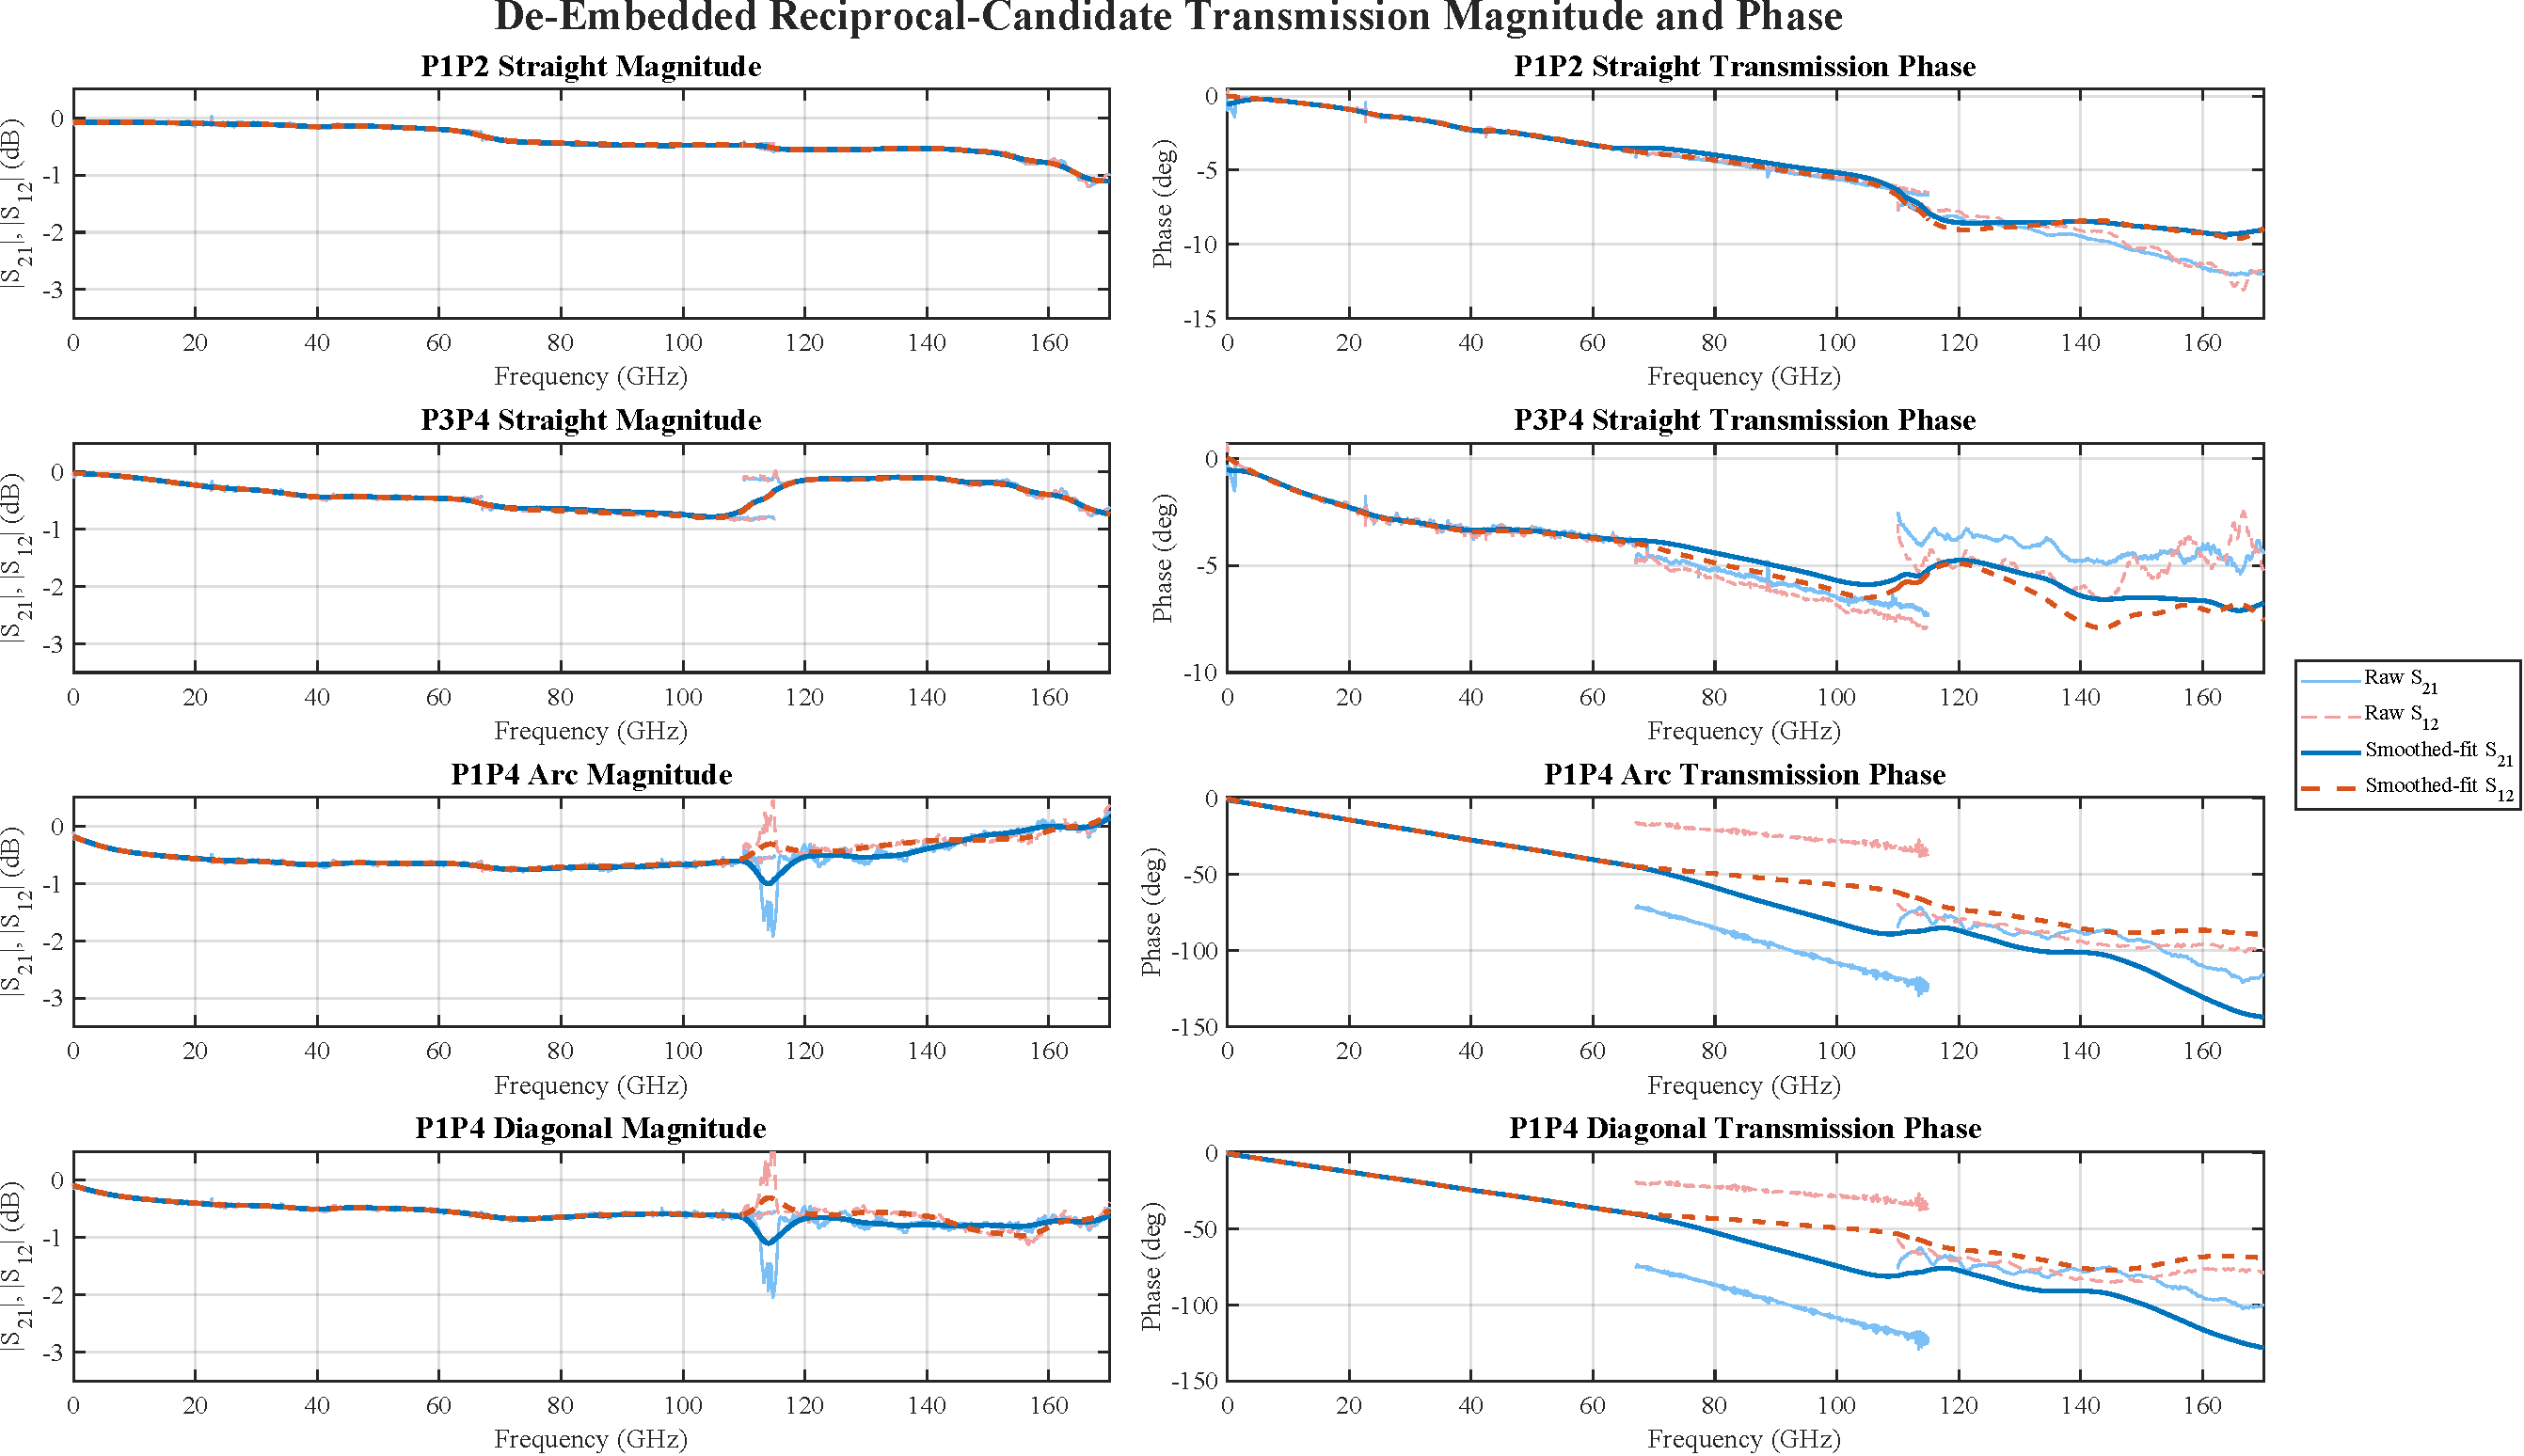
\includegraphics[width=0.98\textwidth]{dissertationResults/outputs/figures/Section5_2_ReciprocalTransmissionAndPhase.pdf}
\caption{De-embedded transmission magnitude and phase of the reciprocal-standard candidates after removal of the common embedding extracted from the straight Thru. Each row corresponds to one reciprocal candidate, with \(S_{21}\) and \(S_{12}\) magnitude shown on the left and the corresponding transmission phase shown on the right. The P1P2 straight Thru remains the cleanest collinear benchmark with full-span mean reciprocity mismatch 0.0033, median insertion loss 0.458~dB, and phase-ripple RMS 0.509$^\circ$, while the P3P4 straight cross-check gives 0.0089, 0.384~dB, and 1.168$^\circ$. Among the orthogonal candidates, the arc is preferred to the diagonal because it gives lower full-span reciprocity mismatch (0.3121 versus 0.3199), lower median insertion loss (0.591~dB versus 0.599~dB), and much lower phase-ripple RMS (1.467$^\circ$ versus 4.971$^\circ$).}
\label{fig:sec52_recip_transmission}
\end{figure*}

Figure~\ref{fig:sec52_recip_transmission} summarizes the de-embedded transmission responses of the reciprocal candidates. Over the full 0.01--170~GHz span, the P1P2 straight Thru gives mean reciprocity mismatch 0.0033, median insertion loss 0.458~dB, and phase-ripple RMS 0.509$^\circ$, making it the cleanest collinear benchmark. The independent P3P4 straight structure gives mean reciprocity mismatch 0.0089, median insertion loss 0.384~dB, and phase-ripple RMS 1.168$^\circ$, so it remains a useful cross-check but is less well behaved than the primary P1P2 straight reference. The two orthogonal candidates are clearly poorer than the straight references, particularly above 110~GHz, and must therefore be assessed directly from their measured reciprocal behavior rather than by geometric intuition.

The numerical comparison is summarized in Table~\ref{tab:sec52_recip_summary}. Between the two orthogonal structures, the arc yields full-span mean reciprocity mismatch 0.3121 versus 0.3199 for the diagonal, median insertion loss 0.591~dB versus 0.599~dB, and phase-ripple RMS 1.467$^\circ$ versus 4.971$^\circ$. The diagonal gives the better median worst-port return loss, 18.70~dB versus 13.62~dB for the arc, but the transmission-standard decision is governed more strongly by reciprocity and phase smoothness than by return loss alone. The same pattern is visible in the bandwise rows of Table~\ref{tab:sec52_recip_summary}: in 67--115~GHz the arc and diagonal have similarly large reciprocity mismatch, 1.0920 and 1.0993, while the arc retains the lower phase-ripple RMS, 0.198$^\circ$ versus 0.271$^\circ$; in 110--170~GHz the arc again gives the lower mismatch, 0.1198 versus 0.1367, and lower phase-ripple RMS, 1.270$^\circ$ versus 1.343$^\circ$, while also preserving lower median insertion loss, 0.331~dB versus 0.682~dB.

\begin{sidewaystable}[p]
\centering
\caption{Measured reciprocal-standard metrics by structure and band after de-embedding to the common standard-definition plane. Reciprocity mismatch is reported as \(\epsilon_{\mathrm{rec}}=\lvert S_{21}-S_{12}\rvert\).}
\label{tab:sec52_recip_summary}
\scriptsize
\setlength{\tabcolsep}{3pt}
\renewcommand{\arraystretch}{1.15}
\begin{tabular}{p{2.35cm}p{2.45cm}p{1.35cm} >{\centering\arraybackslash}p{1.35cm} >{\centering\arraybackslash}p{1.35cm} >{\centering\arraybackslash}p{1.20cm} >{\centering\arraybackslash}p{1.15cm} >{\centering\arraybackslash}p{1.55cm} >{\centering\arraybackslash}p{1.45cm} >{\centering\arraybackslash}p{1.35cm} >{\centering\arraybackslash}p{1.15cm}}
\hline
Structure & Role & Band & \shortstack{Mean\\\(\epsilon_{\mathrm{rec}}\)} & \shortstack{Max\\\(\epsilon_{\mathrm{rec}}\)} & \shortstack{Median\\IL (dB)} & \shortstack{Max\\IL (dB)} & \shortstack{Median\\worst-port\\RL (dB)} & \shortstack{Min\\worst-port\\RL (dB)} & \shortstack{Phase\\ripple RMS\\(deg)} & \shortstack{Repeat-\\ability} \\
\hline
P1P2 Straight & Straight benchmark & 0--67 & 0.0008 & 0.0240 & 0.125 & 0.269 & 29.12 & 22.88 & 0.128 & N/E \\
P1P2 Straight & Straight benchmark & 67--115 & 0.0027 & 0.0101 & 0.468 & 0.501 & 23.50 & 21.47 & 0.063 & N/E \\
P1P2 Straight & Straight benchmark & 110--170 & 0.0063 & 0.0174 & 0.564 & 1.205 & 26.16 & 15.83 & 0.251 & N/E \\
P1P2 Straight & Straight benchmark & Full-span & 0.0033 & 0.0240 & 0.458 & 1.205 & 26.52 & 15.83 & 0.509 & N/E \\
\hline
P3P4 Straight & Straight cross-check & 0--67 & 0.0011 & 0.0240 & 0.347 & 0.507 & 24.05 & 17.82 & 0.373 & N/E \\
P3P4 Straight & Straight cross-check & 67--115 & 0.0073 & 0.0164 & 0.713 & 0.843 & 20.42 & 17.66 & 0.084 & N/E \\
P3P4 Straight & Straight cross-check & 110--170 & 0.0186 & 0.0438 & 0.149 & 0.754 & 23.22 & 16.51 & 0.501 & N/E \\
P3P4 Straight & Straight cross-check & Full-span & 0.0089 & 0.0438 & 0.384 & 0.843 & 22.80 & 16.51 & 1.168 & N/E \\
\hline
P1P4 Arc & Orthogonal candidate & 0--67 & 0.0012 & 0.0228 & 0.624 & 0.726 & 20.49 & 15.71 & 0.172 & N/E \\
P1P4 Arc & Orthogonal candidate & 67--115 & 1.0920 & 1.4648 & 0.698 & 0.780 & 13.51 & 12.67 & 0.198 & N/E \\
P1P4 Arc & Orthogonal candidate & 110--170 & 0.1198 & 0.3601 & 0.331 & 0.889 & 9.54 & 4.25 & 1.270 & N/E \\
P1P4 Arc & Orthogonal candidate & Full-span & 0.3121 & 1.4648 & 0.591 & 0.889 & 13.62 & 4.25 & 1.467 & N/E \\
\hline
P1P4 Diagonal & Orthogonal candidate & 0--67 & 0.0010 & 0.0237 & 0.456 & 0.631 & 22.84 & 17.74 & 0.156 & N/E \\
P1P4 Diagonal & Orthogonal candidate & 67--115 & 1.0993 & 1.4607 & 0.610 & 0.705 & 18.32 & 14.73 & 0.271 & N/E \\
P1P4 Diagonal & Orthogonal candidate & 110--170 & 0.1367 & 0.4063 & 0.682 & 1.013 & 9.48 & 5.69 & 1.343 & N/E \\
P1P4 Diagonal & Orthogonal candidate & Full-span & 0.3199 & 1.4607 & 0.599 & 1.013 & 18.70 & 5.69 & 4.971 & N/E \\
\hline
\end{tabular}
\end{sidewaystable}


On balance, the arc is the better orthogonal reciprocal candidate because it gives lower full-span reciprocity mismatch (0.3121 versus 0.3199), lower full-span median insertion loss (0.591~dB versus 0.599~dB), and much lower full-span phase-ripple RMS (1.467$^\circ$ versus 4.971$^\circ$). The diagonal structure is therefore retained as a cross-check rather than promoted as the primary reciprocal standard. This choice is based on measured de-embedded behavior rather than on layout symmetry or simulation expectations alone.

The main conclusion of this section is therefore that the reciprocal standard must be regarded as a measured transmission standard with finite electrical length, finite loss, and geometry-specific parasitics, not as an abstract ideal thru. Provided that reciprocity is preserved and the measured transmission response remains smooth and well controlled, such a structure is fully compatible with the SOLR framework and is better suited to the orthogonal four-port environment than an ideal-thru assumption. The P1P4 arc reciprocal structure selected in this section is carried forward into Section~5.3 as the measured reciprocal standard used in the experimental implementation of the four-port SOLR routine.
